% Background %

\begin{chapterabstract}
This chapter begins with a comprehensive overview of mutation testing, a fault‐injection technique that quantifies test suite effectiveness by introducing small syntactic changes—mutants—into code and measuring the mutation score (the ratio of killed to generated mutants) to uncover weaknesses beyond traditional coverage metrics \cite{jia2011analysis,offutt1996practical,petrovic2018industrial}. We present Mutatr, an R package for prototype‐based mutable objects—heavily inspired by the Io language and JavaScript—which enables the dynamic creation and manipulation of mutated object states to support custom mutation operators in testing workflows \cite{hadley-mutatr,iolanguage}. We then introduce the R language, highlighting its rich ecosystem for statistical computing and data analysis, and the \texttt{testthat} framework for writing expressive unit tests within R packages \cite{rcore2024,wickham2011testthat}. Finally, we delve into R’s C API internals—focusing on the \texttt{SEXP} type, memory protection, and the traversal of pairlists via \texttt{CAR()}, \texttt{CDR()}, and \texttt{TAG()}—to illustrate how low‐level structures underpin R’s object model \cite{hadley-r-internals-pairlists}.  

\end{chapterabstract}

\section{Mutation Testing}

\subsection{Mutation Testing}

Mutation testing is a technique for evaluating the effectiveness of software test suites by systematically introducing small syntactic modifications—known as mutants—into a program \cite{jia2011analysis}. These mutants are created via a process called mutagenesis, whereby specific mutation operators transform the original code to produce slightly altered versions \cite{offutt1996practical}. The fundamental premise is that an effective test suite should be capable of identifying and \textit{killing} these mutants—causing at least one test to fail when executed against a mutant. If no test fails, the mutant remains \textit{alive}, suggesting potential weaknesses in the test suite. This approach provides a more rigorous assessment of test robustness than traditional code coverage metrics, which merely indicate whether parts of the code have been executed \cite{petrovic2018industrial}.

\subsection{Mutant}

In mutation testing, a mutant refers to a slightly modified version of a software program. These modifications intentionally mimic common faults or errors programmers might make, such as replacing an arithmetic operator (e.g., changing \texttt{+} to \texttt{-}) or altering variable names \cite{jia2011analysis}. The purpose of creating mutants is to test the effectiveness of a software test suite. If a test case fails when executed against a mutant, that mutant is considered \textit{killed}. 

\subsection{Mutation operator}

Mutants are generated using predefined mutation operators, which define the specific rules or types of changes applied to the original code to produce mutants \cite{offutt1996practical}. These operators simulate typical programming mistakes or variations to strengthen test suites. For example, a mutation operator might systematically replace relational operators (\texttt{>} with \texttt{<}) or insert exceptions such as division by zero \cite{jia2011analysis}. Through these operators, developers can create diverse mutants, enhancing the robustness and completeness of their testing strategies.

\subsection{Mutation score}

The effectiveness of a test suite is quantified using a metric known as the mutation score, defined as the proportion of killed mutants relative to the total number of generated mutants \cite{jia2011analysis}. A higher mutation score indicates a more fault-sensitive and robust test suite. However, practical application of mutation testing, especially in large-scale software systems, presents significant computational challenges \cite{petrovic2018industrial}. The necessity to execute the full test suite against each mutant results in substantial computational overhead, particularly in complex packages containing numerous tests. Additionally, the existence of equivalent mutants, which behave identically to the original program despite syntactic changes, complicates mutation testing. These equivalent mutants cannot be killed by any test, potentially deflating the mutation score if not identified correctly \cite{offutt1996practical}.

\subsection{Mutation analysis procedure}

The conventional procedure of mutation analysis is depicted in Figure~\ref{fig:MutationAnalysis}. A set of faulty program versions—mutants, denoted as \( p' \)—is systematically derived from the original program \( p \) through small syntactic modifications guided by predefined mutation operators. For instance, as shown in Table~\ref{tab:MutationOperation}, a mutant \( p' \) can be created by altering a logical AND operator (\texttt{\&\&}) to a logical OR operator (\texttt{||}). This intentional alteration results in behaviorally distinct program versions, which are subsequently tested to evaluate the effectiveness of the existing test suite \cite{jia2011analysis}.

\subsection{Equivalent mutants}

A persistent challenge in mutation testing field is the identification of equivalent mutants, which are syntactically different from the original program but semantically behave the same for all possible inputs. These mutants cannot be detected by any test and thus skew mutation score results, leading to wasted effort in manual inspection or incorrect assessment of test suite quality. Addressing this issue, recent research has explored leveraging the capabilities of large language models (LLMs) for automatic equivalent mutant detection. Tian et al. (2024) conducted a comprehensive study evaluating several LLMs (e.g., GPT-3.5, GPT-4) across diverse programming languages and mutation scenarios. They found that, while LLMs show promise, particularly in tasks where mutants and original code differ clearly in behavior, their performance is still far from being reliable for subtle semantic equivalence cases. The authors also propose a benchmark and evaluation framework for standardized assessment, highlighting the gap between current LLM capabilities and the demands of robust equivalent mutant identification \cite{tian2024large}.

\subsection{Importance}

Mutation testing is recognized as one of the most powerful techniques to evaluate the effectiveness and reliability of test suites in software development. It involves intentionally introducing faults, known as mutants, into a program's source code and determining if the existing tests can detect these faults. If tests fail to detect these mutants, it indicates weaknesses in the test suite, highlighting areas that require improvement.

The industrial importance of mutation testing has been demonstrated notably by Petrovic and Ivankovic in their comprehensive case study conducted at Google \cite{petrovic2018industrial}. Their research evaluated mutation testing on an industrial scale, involving over 30,000 developers and 1.9 million change sets across multiple programming languages. They concluded that mutation testing significantly enhances test suite quality by systematically identifying test coverage deficiencies, although it also poses challenges due to its computational complexity and resource demands. The findings emphasize the practicality and benefit of integrating mutation testing into large-scale, real-world software engineering processes.

\begin{figure}[!htbp]
    \centering
    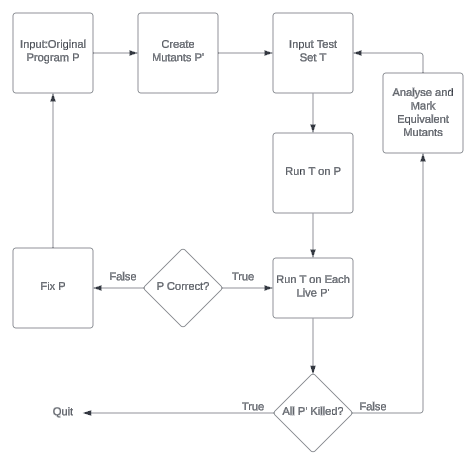
\includegraphics[width=\linewidth]{images/MutationProcess.png}
    \caption{Generic process of mutation analysis.~\cite{offutt2010mutation}}
    \label{fig:MutationAnalysis}
\end{figure}

\begin{figure}[!htbp]
    \centering
    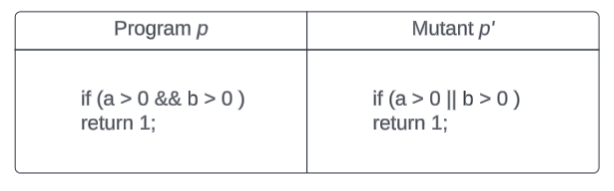
\includegraphics[width=\linewidth]{images/MutationOperation.png}
    \caption{An Example of Mutation Operation ~\cite{offutt2010mutation}.}
    \label{fig:MutationOperation}
\end{figure}

\subsection{Mutatr}

Mutatr is an R package providing prototype‐based mutable objects, enabling in‐memory mutation of R object state without altering the original prototypes \cite{hadley-mutatr}. Inspired by the Io language and JavaScript’s object model, it offers a concise API for defining prototypes, cloning them, and applying direct field mutations—features that can be leveraged to implement custom mutation operators or to generate dynamic test fixtures in R-based mutation testing pipelines \cite{iolanguage}.

\begin{verbatim}
# Install Mutatr from GitHub
if (!requireNamespace("devtools", quietly = TRUE)) {
  install.packages("devtools")
}
devtools::install_github("hadley/mutatr")

library(mutatr)

# Define a simple prototype with initial state
proto <- mutatr::prototype(list(count = 0, flag = TRUE))

# Clone the prototype and apply mutations
mutant <- clone(proto)
mutant$count <- mutant$count + 1
mutant$flag  <- FALSE

# Inspect mutated object
print(mutant)
\end{verbatim}

By integrating Mutatr-driven object mutations into test suites—e.g., verifying that functions behave correctly when object state changes—developers can extend traditional code-level mutation testing with stateful, object-oriented mutation scenarios.

\section{R language}

\subsection{R language}

R is a widely-used open-source programming language designed primarily for statistical computing, data analysis, and graphical visualization \cite{rcore2024}. Due to its extensive package ecosystem and versatility, R has become one of the leading tools for exploratory data analysis, predictive modeling, and reproducible research \cite{wickham2014advanced}. Its rich syntax enables users to express complex analytical workflows concisely, facilitating rapid prototyping and iterative development \cite{wickham2019r4ds}. For example, the following R script generates a simple scatter plot:

\begin{verbatim}
# Load required package
library(ggplot2)

# Create sample data
df <- data.frame(
  x = 1:10,
  y = runif(10)
)

# Plot data
ggplot(df, aes(x = x, y = y)) +
  geom_point() +
  labs(
    title = "Sample Scatter Plot",
    x = "X-axis",
    y = "Y-axis"
  )
\end{verbatim}

This snippet demonstrates how easily R can be used for data visualization \cite{wickham2019r4ds}.

\subsection{testthat library}

The \texttt{testthat} package is an R library specifically designed to simplify and encourage automated software testing practices \cite{wickham2011testthat}. Developed by Hadley Wickham, it has become the most widely used testing framework within the R community. \texttt{testthat} provides a straightforward and expressive syntax, allowing developers to clearly articulate test expectations and quickly verify the correctness of their functions. For instance, a simple unit test using \texttt{testthat}:

\begin{verbatim}
# Example function to add two numbers
add <- function(a, b) {
  a + b
}

# Unit test for 'add' function
library(testthat)

test_that("add returns correct sum", {
  expect_equal(add(1, 2), 3)
  expect_type(add(1, 2), "double")
})
\end{verbatim}

By supporting unit testing and test-driven development, \texttt{testthat} enhances software reliability and encourages developers to rigorously consider the behavior of their code. It integrates seamlessly into the standard R package development workflow, facilitating continuous integration, debugging, and reproducible test suites \cite{wickham2015rpackages}.

\subsection{R package structure}

A typical R package follows a standardized directory layout to ensure consistency and reproducibility \cite{wickham2015rpackages}. At a minimum, an R package contains:

\begin{verbatim}
PackageName/
  DESCRIPTION
  NAMESPACE
  R/
    functions.R
  man/
    functions.Rd
  tests/
    testthat/
      test-functions.R
\end{verbatim}

The \texttt{DESCRIPTION} file provides metadata such as package name, version, and dependencies, while \texttt{NAMESPACE} declares exported functions. The \texttt{R/} directory holds R scripts with function definitions, and \texttt{man/} contains documentation in \texttt{.Rd} format. Test files reside in \texttt{tests/testthat/}, enabling automated testing with \texttt{testthat}.

\subsection{R C API}

For performance-critical code, R allows integration of C routines through its R C Application Programming Interface (API) \cite{rcore2024}. Central to this interface is the \texttt{SEXP} type, an opaque pointer representing R objects in C. Proper memory management requires the use of \texttt{PROTECT} and \texttt{UNPROTECT} to guard against garbage collection. For example, a C function to sum elements of a numeric vector:

\begin{verbatim}
// sum.c
#include <R.h>
#include <Rinternals.h>

// Sum a numeric vector from R
SEXP c_sum(SEXP vector) {
  // Ensure input is numeric
  PROTECT(vector = coerceVector(vector, REALSXP));
  int n = length(vector);
  double *v = REAL(vector);
  double total = 0.0;

  for (int i = 0; i < n; i++) {
    total += v[i];
  }

  // Create result
  SEXP result = PROTECT(allocVector(REALSXP, 1));
  REAL(result)[0] = total;

  UNPROTECT(2); // vector and result
  return result;
}
\end{verbatim}

This routine can be compiled and called from R via the \texttt{.Call} interface, providing significant speedups for large-scale numerical operations \cite{rcore2024}.

In R’s internal C API, pairlists are the fundamental data structure used to represent any ordered collection of tagged elements—most notably, argument lists for function calls (`LANGSXP`), the special `...` object (`DOTSXP`), and attribute lists on objects (`LISTSXP`) \cite{hadley-r-internals-pairlists}.  Under the hood, each pairlist is implemented as a singly linked list of CONS cells, where each cell holds:

\begin{itemize}
  \item \texttt{CAR(p)}: the payload, an \texttt{SEXP} that points to the actual R object stored in that position;
  \item \texttt{CDR(p)}: a pointer to the next CONS cell in the list (or \texttt{R\_NilValue} when you’ve reached the end);
  \item \texttt{TAG(p)}: an optional name (a symbol) for the element, used when the list represents named arguments or named attributes.
\end{itemize}

Visiting every element in such a list is straightforward: you begin at the head \texttt{SEXP} and follow the \texttt{CDR()} pointer repeatedly until you encounter \texttt{R\_NilValue}.  At each step, you can inspect the current element’s value via \texttt{CAR()}, and if the list is named, examine the tag via \texttt{TAG()}.  A typical traversal loop looks like:

\begin{verbatim}
for (SEXP node = plist; node != R_NilValue; node = CDR(node)) {
  SEXP elt = CAR(node);        // current element
  SEXP name = TAG(node);       // may be R_NilValue if unnamed
  // process 'elt' and, if 'name' != R_NilValue, CHAR(PRINTNAME(name))
}
\end{verbatim}

This pattern is used for everything from counting elements to inspecting argument names in a call.  For example, to count the elements:

\begin{verbatim}
// Count the number of elements in a pairlist
int pairlist_length(SEXP plist) {
  int count = 0;
  for (SEXP node = plist; node != R_NilValue; node = CDR(node)) {
    count++;
  }
  return count;
}
\end{verbatim}

If you need random access to the \(n\)th element, R provides the helper function \texttt{Rf\_nthcdr(plist, n)}, which returns the sublist starting at position \(n\) (zero‐based).  However, beware: repeatedly calling \texttt{Rf\_nthcdr} inside a loop can degrade to \(O(n^2)\) time complexity for long lists, since each call walks from the head \cite{hadley-r-internals-pairlists}.  

When handling function calls in C, you often want to skip the first element (the function symbol) and traverse only the arguments:

\begin{verbatim}
// Print each argument name and its type for a call object
void print_call_args(SEXP call) {
  SEXP args = CDR(call);  // skip function name at CAR(call)
  for (SEXP arg = args; arg != R_NilValue; arg = CDR(arg)) {
    SEXP tag = TAG(arg);
    const char *argname = (tag != R_NilValue)
                          ? CHAR(PRINTNAME(tag))
                          : "<unnamed>";
    SEXP val = CAR(arg);
    Rprintf("Argument '%s' has type %s\n",
            argname,
            type2char(TYPEOF(val)));
  }
}
\end{verbatim}

In this way, you can both retrieve the value and the associated name of each argument in the call.  This canonical looping structure—advance by \texttt{CDR()}, inspect via \texttt{CAR()}, and optionally read or modify the tag via \texttt{TAG()} or \texttt{SET\_TAG()}—applies uniformly to all pairlist‐based data in the R internals API \cite{hadley-r-internals-pairlists}.
